\chapter{Regular Expression Synthesis}

\begin{figure}[t]
  \centering
  \pgfdeclarelayer{background}   % layer with the synthesizer rectangle
  \pgfsetlayers{background,main} % background behind main
  
  
    \begin{tikzpicture}[%
  auto,
  trim left=(decider), trim right=(decider)
] %, trim right=(spec)]

  \node (centre) at (0,0) {};

  \node[square] (enumerator) [above=of centre, yshift=-.2cm] {Enumerator};

  \node[square] (decider)   [below=of centre, yshift=.2cm] {Decider};

  \node[nosquare] (DSL) [above=0.5 of enumerator] {\ac{DSL}};

  
  \node[square] (distinguisher) [below = 1.5 and 1 of decider, align=center]
  {Distinguisher};
  
  \node[square] (user) [below left = .3 and 2.3 of decider]
  {User};
  
  \node[nosquare] (valid) [right=2.7 of distinguisher, align=left] {%
    \textbf{Desired}\\ \textbf{Program}%
  };

  
  \draw [arrow] (enumerator.240) to node[left=.5mm,align=right, text width=1.9cm] (candidate) {Candidate\\program} (decider.120);

  \draw [arrow] (decider.60) to node[right=.5mm, align=left, text width=1.9cm]  (failure) {Reason\\of failure}  (enumerator.300);

  \draw [arrow] (DSL) to (enumerator);

  \draw [arrow] (distinguisher) to [align=center, below] node (unsat) {Correct\\program} (valid);
  
  \draw [arrow] (decider) to node [align=left, right] (p1p2) {2 correct\\programs}
  (distinguisher);
  
  \draw [arrow] (user)    |- node [above, near end, align=center] (io_examples) {Input-output\\examples} (decider);
  
  \draw [arrow] (distinguisher) -| node [below, near start, align=center] (dist_input) { Distinguishing\\input} (user);
  
  %\draw [arrow] (distinguisher.west) to node [align=right, below=.3] (dist_input) {%
  %  distinguishing input%
  %} (user);

  
  \begin{pgfonlayer}{background}
    \path let \p1=(DSL.north west),
              \p2=(enumerator.west)
    in
      coordinate (topleftcorner) at (\x2, \y1);
      
    \path let \p1=(distinguisher.south),
              \p2=(enumerator.east)
    in
      coordinate (bottomrightcorner) at (\x2, \y1);
      
    \path let \p1=(topleftcorner),
              \p2=(bottomrightcorner)
    in
      coordinate (toprightcorner) at (\x2, \y1);
    
    % gre grey square representing synth's domain
    \draw[enclosing_square] (synth)
      ($(topleftcorner)+(-1.5,0.6)$) rectangle
      ($(bottomrightcorner)+(1.5,-.6)$);
    
    \node[gray,nosquare, anchor=north east] (synthtext) at ($(toprightcorner)+(1.1cm, 0.5cm)$) {Synthesizer};
  \end{pgfonlayer}

  \end{tikzpicture}

  \caption{Complete Synthesizer}
  \label{fig:synthesizer}
\end{figure}

The task of automatically generating a program that satisfies some desired behavior expressed as a high-level specification is known as Program Synthesis. \acf{PBE} is a branch of Program Synthesis where the desired behavior is specified using input-output examples. 
%
Before the synthesis procedure starts, we define the set of operators that can be used to build the desired regex, as well as the values each operator can take as argument. These constitute the synthesizer's \ac{DSL}. \Forest{} builds its DSL based on the user-provided examples. Each DSL is dynamically constructed to fit the problem at hand: it is as restricted as possible, without losing any expressiveness necessary to ensure it includes the correct regex. The DSL construction procedure is detailed in \autoref{sec:dsl}.

\begin{figure}[t]
  \centering
  \pgfdeclarelayer{background}   % layer with the synthesizer rectangle
  \pgfsetlayers{background,main} % background behind main
  
  
    \begin{tikzpicture}[%
  auto,
  trim left=(user), trim right=(user)
] %, trim right=(spec)]
  \sffamily
  
  \node[square] (verifier) {Verifier};

  \node[square] (enumerator) [above=1 of verifier] {Enumerator};

  \node[nosquare] (DSL) [above=0.3 of enumerator] {DSL};
  
  \node [nosquare, black, font=\bf\sffamily] (io_examples) [left=1.5 of verifier, align=center] {I/O\\examples};
  
  \node[square] (distinguisher) [right=1.5 of verifier, align=center]
  {Distinguisher};
  
  \node (user) [below right=.7 and 0.2 of verifier]
  {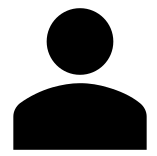
\includegraphics[width=1cm]{pictures/user2.png}};
  
  \node[nosquare] (desired) [black, font=\bf\sffamily, right=1.5 of distinguisher, align=center] {Desired\\Program};

  
  \draw [arrow, bend right=45] (enumerator) to  node[align=center, left] (candidate) {candidate\\program} (verifier);

  \draw [arrow, bend right=45] (verifier) to node[align=center, right]  (failure) {reason\\of failure}  (enumerator);

  \draw [arrow] (DSL) to (enumerator);
  
  \draw [arrow] (io_examples) to (verifier);

  \draw [arrow] (distinguisher)  to [align=left, right] node (unsat) {} (desired);
  
  \draw [arrow] (verifier) to node [align=center, below] (p1p2) {2 correct\\programs}
  (distinguisher);
  
  \draw [arrow,  bend left=30] (user.170) to node [left=.3, align=center, near start] (new_io_example) {new I/O\\example} (verifier.south);
  
  \draw [arrow, bend left=30] (distinguisher.south) to node [right=.2, align=center, near end] (dist_input) {new\\input} (user.10);
  

  
  %\draw [arrow] (distinguisher.west) to node [align=right, below=.3] (dist_input) {%
  %  distinguishing input%
  %} (user);

  
  \begin{pgfonlayer}{background}
    \path let \p1=(enumerator.west),
              \p2=(DSL.north)
    in
      coordinate (topleftcorner) at (\x1, \y2);
      
    \path let \p1=(distinguisher.east),
              \p2=(p1p2.south)
    in
      coordinate (bottomrightcorner) at (\x1, \y2);
      
    \path let \p1=(topleftcorner),
              \p2=(bottomrightcorner)
    in
      coordinate (toprightcorner) at (\x2,\y1);
    
    % gre grey square representing synth's domain
    \draw[enclosing_square]
      ($(topleftcorner)+(-1.2,.1)$) rectangle
      ($(bottomrightcorner)+(1,-.1)$);
    
    \node[synth_node, anchor=north west] (synthtext) at ($(toprightcorner)+(-0.9,0)$) {Synthesizer};
  \end{pgfonlayer}

  \end{tikzpicture}

  \caption{Interactive synthesis algorithm.}
  \label{fig:interactive-synthesis}
\end{figure}

Our synthesis algorithm employs enumerative search, a very common approach to solve the problem of program synthesis \cite{DBLP:conf/pldi/FengMBD18,DBLP:conf/pldi/FengMGDC17,AlphaRegex16,Orvalho19,DBLP:conf/cav/ReynoldsBNBT19}. The enumeration cycle finds regexes that are consistent with the user-provided examples. In order to choose an expression among those generated by the enumeration,  \Forest{} interacts with the user. The result of each interaction is a new input-output example that strengthens the original specification. Both the enumeration and the interaction cycle are depicted in \autoref{fig:interactive-synthesis}.

There are two key components for enumerative search: the \textit{enumerator} and the \textit{verifier}.
The \textit{enumerator} successively enumerates regexes from the DSL, while the \textit{verifier} subsequently checks whether they satisfy all the provided examples.
%
Following the Occam's razor principle, regexes are enumerated in increasing order of complexity, so that simpler expressions are evaluated first. %and only after those having been refuted by the \textit{verifier} are more complex expressions considered. 

If the regex does not satisfy the examples, then it can be discarded. If, on the other hand, a regex that is consistent with the user-provided examples is found, it is stored by the synthesizer.
Program synthesis applications generate very large search spaces; however, the search space can be significantly reduced by pruning several infeasible expressions along with each incorrect expression found. 
%These programs can be equivalent to the incorrect program, or sure to fail in the same way as the incorrect program.
%When the \textit{verifier} rejects a regex, the \textit{enumerator} can eliminate from the search space not only the rejected expression but also others that are guaranteed to fail as well. 
The enumeration and pruning processes are further described in \autoref{sec:enumeration}.

As mentioned before, input-output examples are an ambiguous specification. Thus, the synthesizer does not return the first regex consistent with the examples that it finds, as it may not correspond to the user's intended behavior. Instead, \Forest{} provides an interaction model implemented through the \textit{distinguisher} component. Given two regexes, the \textit{distinguisher} ascertains whether they are equivalent. If they are not equivalent, it produces a distinguishing input: a string matched by one of the regexes but not the other. This new input is shown to the user, who classifies it as valid or invalid, effectively choosing one regex over the other. The new input-output pair is added to the examples, and the enumeration process continues. This interactive cycle is further described in \autoref{sec:interaction}. 


\section{\acf{DSL}}\label{sec:dsl}
Before the synthesis procedure starts, the \ac{DSL} of the enumerated regexes must be defined. This includes the definition of the operators that can be used to build the desired regex, as well as the values each operator can take as~argument. 

\Forest{} aims at producing a regular expression that fully  matches the strings provided as valid examples. We consider a successful match only when the regular expression matches the entire string.% This is equivalent to adding ``\verb-^-'' to the beginning and ``\verb-$-'' to the end of the regular expression.

To construct the regex, the \ac{DSL} always includes the union %(\verb-|-)
and concatenation operators. The union of two arbitrary regexes \(r\) and \(s\) creates a new regex, denoted \(r|s\). A string matches \(r|s\) if it matches \(r\) or \(s\). Similarly, the concatenation of any two regexes \(r\) and \(s\), creates a new regex, \(rs\). If a string \(p\) is matched by \(r\) and a string \(q\) is matched by \(s\), then \(pq\) is matched by \(rs\).

In addition, we consider several regular expression quantifiers. A quantifier can be applied to any regex \(r\) and is equivalent to concatenating \(r\) with itself a certain number of times. The \ac{DSL} includes the following quantifiers:
\begin{itemize}[topsep=0pt]
    \item \textit{Kleene} closure (*), which matches 0 or more times,
    \item positive closure (+), which matches 1 or more times,
    \item option (?), which matches 1 or 0 times,
    \item range (\(\{m\}\)), which matches exactly \(m\) times, and
    \item range (\(\{m,n\}\)), which matches at least \(m\) times and at most \(n\) times.
\end{itemize}

\noindent
The possible values for the range operators are limited depending on the valid examples provided by the user. For the single-valued range operator, \(\{m\}\), we consider only the integer values such that \(2 \le m \le l\), where \(l\) is the length of the longest valid example string. Note that \(m = 1\) is not considered since it is the identity function (\(r\)\(\{1\}\) = \(r\)).
In the two-valued range operator, \(\{m,n\}\), the values of \(m\) and \(n\) are limited to integers such that \(0 \le m < n \leq l\), where \(l\) is again the length of the longest valid example string. The tuple (0,1) is not considered, since its semantics are equivalent to that of the option quantifier:~\(r\{0,1\} = r?\).


All operators can be applied to regex literals or composed with each other to form more complex expressions.
The regex literals considered in the synthesis procedure also depend on the valid input examples. These include the individual letters, digits or symbols present in the examples and all character classes that include them.
The character class \texttt{[\(r_1\)-\(r_n\)]} is shorthand for the regular expression  \texttt{\(r_1\)|\(r_2\)|...|\(r_n\)}, when \(r_1 r_2 ... r_n\) form a logical sequence.
The character classes contemplated in the DSL are \texttt{[0-9]}, \texttt{[A-Z]}, \texttt{[a-z]} and all combinations of those, such as \texttt{[A-Za-z]} or \texttt{[0-9A-Za-z]}. Additionally, \texttt{[0-9A-F]} and \texttt{[0-9a-f]} are used to represent hexadecimal numbers.

The DSL can be represented as a \ac{CFG}. A \ac{CFG} is defined by a 4-tuple \((N, \Sigma, R, S)\), where \(N\) is a set of non-terminal symbols, \(\Sigma\)~a~set of terminal symbols (disjoint from \(N\)), and \(R\) a set of rules or productions, each of the form \(A \to \beta\), where \(A\) is a non-terminal and \(\beta\) is a string of symbols from the set \((\Sigma \cup N)*\). \(S \in N\) is the designated start symbol.
The terminal symbols \(\Sigma\) include the names of all regex operators, as well as the regex literals and the range operator values.
\(N\), the non-terminal symbols, are the data~types in the~DSL.

\begin{example}\label{ex:dsl}
The literal values on the DSL depend on the input examples.
% Recall \autoref{ex:1}, where the valid input values were:

% \begin{multicols}{3}
%     \begin{itemize}[label={},topsep=0em]
%     \item 19/08/1996
%     \item 26/10/1998
%     \item 22/09/2000
%     \item 01/12/2001
%     \item 29/09/2003
%     \item 31/08/2015
%     \end{itemize}
% \end{multicols}
%\noindent
%
Consider the valid examples in \autoref{ex:1}.
%
In this scenario, the length of the longest valid example is \(l = 10\), so the range value literals are \(m \in \{2, ..., 10\}\), for the single valued range, and \((n, m): 0 \leq n < m \leq 10\) for the two-valued range. The characters in the examples are `/', which becomes itself a regex literal, and digits, which introduce the character class \texttt{[0-9]}. The \ac{CFG} is then defined as shown in \autoref{fig:dsl}.
%
\end{example}
\begin{figure}[t]
  \begin{align*}
    Re \;\to \;\;&  \Concat(Re, Re) \;\;|\;\;  \Union(Re, Re)   \;\;|\;\;  \Kleene(Re) \;\;|\;\;  \Posit(Re) \\
          |\;\;&  \Option(Re) \;\;|\;\;  \Range(Re, \Rangelit) \;\;|\;\; \texttt{[0-9]} \;\;|\;\; \texttt{/}\\
    \Rangelit \;\to \;\;&  2 \;|\; 3 \;|\; ... \;|\; 10 \;|\; (0,2) \,|\, (1,2)\,|\, (0,3) \,|\, ... \,|\, (8,10)\,|\, (9,10)
  \end{align*}
  \captionsetup{belowskip=-7pt, aboveskip=-5pt}
  \caption{\ac{CFG} that represents the \ac{DSL} of regular expressions for \autoref{ex:1}. \(Re\) is the start symbol and the representation of the regex type, \(\Rangelit{}\) represents the possible values for the argument of the range operator.}
  \label{fig:dsl}
\end{figure}



\section{Synthesis Algorithm}\label{sec:enumeration}

To enumerate regexes, the synthesizer requires a structure capable of representing every feasible expression. % There are different approaches to achieve this. 
Orvalho et. al. \cite{Orvalho19} describe two different representations: tree-based and line-based. The tree-based representation follows a typical hierarchical composition of operations, as usually seen in functional languages, while the line-based representation emulates the structure of a program written in an imperative language, where each operation is seen as a line of code.

We opt to use a tree-based representation of the search space, using \(k\)-trees. A \(k\)-tree of depth \(d\) is a tree in which every internal node has exactly \(k\) children and every leaf node is at depth \(d\).
If \(k\) is the greatest arity among all DSL constructs, then a \(k\)-tree of depth \(d\) can represent all programs of depth up to \(d\) in that \ac{DSL}. For that, a symbol of the DSL is assigned to each node and the tree can be interpreted as a program. In any regex DSL built by \Forest{}, the maximum arity is always 2, so all regexes in the search space can be represented using 2-trees. In \autoref{fig:date-ktree}, the regex from \autoref{ex:1}, \UseVerb{date2}, is represented as a 2-tree of depth 5.

To explore the search space in order of increasing complexity, the \(k\)-tree enumerator starts by analysing trees of lower depths and progressively increases the depth of the tree as trees of previous depths are exhausted.
%We start with a tree of depth \(d=1\). Only if no solution is found with depth 1, does the synthesizer proceed to enumerate trees of depth \(d=2\), and so on.
This way we ensure the first regex found is of the smallest depth possible.


\begin{figure}[t]
\centering
\begin{tikzpicture}[
level distance=1.1cm,
level 1/.style={sibling distance=6cm},
level 2/.style={sibling distance=3.6cm},
level 3/.style={sibling distance=1.7cm},
level 4/.style={sibling distance=1.1cm,level distance=.9cm}]
\tikzstyle{every node}=[circle,draw,minimum size=1.4pt]
\tikzstyle{every label}=[rectangle, draw=none]

\node (Root) [label={concat}] {}
child {
    node [label={concat}] {} 
    child {
        node [label={concat}] {} 
        child {
            node [label={range}] {} 
            child { node [label=below:{\Verb![0-9]!}] {} }
            child { node [label=below:{2}] {} }
        }
        child {
            node [label={\texttt{/}}] {} 
            child { node [label={[text=eps-node-color]below:\(\epsilon\)}, draw=eps-node-color, right=.08cm] {} edge from parent[draw=eps-node-color] }
            child { node [label={[text=eps-node-color]below:\(\epsilon\)}, draw=eps-node-color, left=.08cm] {} edge from parent[draw=eps-node-color] }
        }
    }
    child {
        node [label={concat}] {} 
        child {
            node [label={range}] {} 
            child { node [label=below:{\Verb![0-9]!}] {} }
            child { node [label=below:{2}] {} }
        }
        child {
            node [label={\texttt{/}}] {} 
            child { node [label={[text=eps-node-color]below:\(\epsilon\)}, draw=eps-node-color, right=.08cm] {} edge from parent[draw=eps-node-color] }
            child { node [label={[text=eps-node-color]below:\(\epsilon\)}, draw=eps-node-color, left=.08cm] {} edge from parent[draw=eps-node-color] }
        }
    }
}
%
child {
    node [label={range}] {} 
    child {
        node [label={\Verb![0-9]!}, right=.3cm] {}
        child {
            node [label={[text=eps-node-color]:\(\epsilon\)}, draw=eps-node-color, right=0cm] {} edge from parent[draw=eps-node-color]
            child { node [label={[text=eps-node-color]below:\(\epsilon\)}, draw=eps-node-color, right=.08cm] {} edge from parent[draw=eps-node-color] }
            child { node [label={[text=eps-node-color]below:\(\epsilon\)}, draw=eps-node-color, left=.08cm] {} edge from parent[draw=eps-node-color] }
        }
        child {
            node [label={[text=eps-node-color]:\(\epsilon\)}, draw=eps-node-color, left=0cm] {} edge from parent[draw=eps-node-color]
            child { node [label={[text=eps-node-color]below:\(\epsilon\)}, draw=eps-node-color, right=.08cm] {} edge from parent[draw=eps-node-color] }
            child { node [label={[text=eps-node-color]below:\(\epsilon\)}, draw=eps-node-color, left=.08cm] {} edge from parent[draw=eps-node-color] }
        }
    }
    child {
        node [label={4}, left=.3cm] {}
        child {
            node [label={[text=eps-node-color]:\(\epsilon\)}, draw=eps-node-color, right=0cm] {} edge from parent[draw=eps-node-color]
            child { node [label={[text=eps-node-color]below:\(\epsilon\)}, draw=eps-node-color, right=.08cm] {} edge from parent[draw=eps-node-color] }
            child { node [label={[text=eps-node-color]below:\(\epsilon\)}, draw=eps-node-color, left=.08cm] {} edge from parent[draw=eps-node-color] }
        }
        child {
            node [label={[text=eps-node-color]:\(\epsilon\)}, draw=eps-node-color, left=0cm] {} edge from parent[draw=eps-node-color]
            child { node [label={[text=eps-node-color]below:\(\epsilon\)}, draw=eps-node-color, right=.08cm] {} edge from parent[draw=eps-node-color]}
            child { node [label={[text=eps-node-color]below:\(\epsilon\)}, draw=eps-node-color, left=.08cm] {} edge from parent[draw=eps-node-color]}
        }
    }
};

\end{tikzpicture}
\caption{\UseVerb{date2} represented as a \(k\)-tree.}
\label{fig:date-ktree}
\end{figure}{}


To explore the space of trees, the enumerator encodes the \(k\)-tree as an SMT formula. 
%
The constraints in the SMT formula ensure that the program is well-typed. 
%
A model that satisfies the formula represents an assignment of a DSL symbol to each tree node. This assignment is then used to build a valid regex. Due to space constraints we omit the \(k\)-tree encoding but further details can be found in appendix \ref{sec:ktree} and in the literature~\cite{DBLP:conf/sigsoft/ChenMF19,Orvalho19}.

%the work of Chen et al.~\cite{DBLP:conf/sigsoft/ChenMF19} and Orvalho et al.~\cite{Orvalho19}.


%Then, a model that satisfies the formula represents an assignment of a DSL symbol to each tree node. This assignment is then used to build a valid regex. \textcolor{red}{The \(k\)-tree encoding is omitted from this document. It is described in \cite{DBLP:conf/sigsoft/ChenMF19} or \cite{Orvalho19}}
%SMT formula such that any assignments that satisfy it correspond to a valid program in the DSL.

\subsection{K-tree encoding}

In this section we offer a formal description of the \(k\)-tree encoding, as proposed by Chen et. al. \cite{DBLP:conf/sigsoft/ChenMF19}.
Consider a \(k\)-tree of depth \(d\). Assume each node in the \(k\)-tree is assigned a unique positive integer index consistent with level-order traversal. Let \(N\) be the set all nodes' indices, \(N = \{1, 2, ..., k^d - 1\}\).
%
Let \(L\) be the set of indices that correspond to leaf nodes and \(I\) the set of indices of internal nodes. Thus \(N = I \cup L\). Furthermore, let \(C(i)\) represent the indices of all children of node \(i\).

Let \(id: \Sigma \to \mathbb{N}\) be a one-to-one mapping of each terminal symbol (i.e., operators and literals) in the DSL to a positive integer.
Because the arity of some DSL operations is smaller than \(k\), there are some children nodes that cannot be assigned any symbol. We introduce the empty symbol, \(\epsilon\), with \(id(\epsilon) = 0\), which is assigned to nodes without symbols.

\paragraph{Encoding variables.}
We define an integer variable \(n_i\) for all \(i \in N\). Assigning \(n_i = id(k)\) means
that we assign the symbol~\(k\) to node \(i\).

\medskip

Next, we add constraints over these variables that ensure the generated regular expression is well-typed. All examples in the remainder of this section refer to the DSL presented in \autoref{ex:dsl} built for the problem described in \autoref{ex:1}.

\paragraph{Leaf constraints.} 
Because they have no children, the leaf nodes must be empty or assigned to a literal of the DSL.
Let \(T\) be the union of \(\epsilon\) with the set of terminal symbols in the DSL that correspond to literals.

\begin{equation}
    \bigwedge_{i \in L} \; \bigvee_{p \in T} n_i = id(p)
\end{equation}

\begin{example}\label{ex:leaf-constraints}
For each leaf node \(i\) we add the constraint:
\begin{gather*}
    n_i = id(\texttt{[0-9]}) \lor n_i = id(\texttt{/}) \lor n_i = id(2) \lor ... \lor n_i = id(10) \lor n_i = id((0,2)) \;\lor \\
    \lor\; n_i = id((1,2)) \lor  n_i = id((0,3)) \lor ... \lor  n_i = id((8,10))\lor  n_i = id((9,10)) 
\end{gather*}
\end{example}


\paragraph{Children constraints.}
If a DSL symbol \(p\) is assigned to a node \(i\), the children of \(i\), \(C(i)\), must have types consistent with the parameters of \(p\).
For each \(p \in \Sigma\) and \(j \in \{1, ..., k\}\), where \(k\) is the largest arity among all DSL constructs, we define \(T(p, j)\).
If \(p\) corresponds to an operator, \(T(p, j)\) denotes the type of parameter \(j\) of \(p\). If \({j > arity(p)}\), then \(T(p,j) = \epsilon\).
If \(p\) represents a literal, then \(T(p,j) = \epsilon\) for every~\(j\).
Finally, let \(\Sigma(T(p,j)) \subset \Sigma\) be the set of terminal symbols in the \ac{DSL} that have type \(T(p,j)\).

\begin{equation}
    \bigwedge_{p \in \Sigma, i \in I}\; \left(n_i = id(p) \Rightarrow \bigwedge_{j \in C(i)} \; \bigvee_{t \in \Sigma(T(p,j))} n_j = id(t) \right)
\end{equation}

\begin{example}\label{ex:children-constraints}
If node 1 is assigned \(\Range\), then its children, nodes 2 and 3, must be assigned symbols of types consistent with its parameters. \({T(\Range, 1) = Re}\), so \(n_2\) must be assigned one of the symbols in
\(\Sigma(Re)=\{\Union, \Concat,\allowbreak \Kleene,\allowbreak \Posit,\allowbreak \Option,\allowbreak \Range, \texttt{[0-9]}, \texttt{/}\}\).
\(T(\Range, 2) = \Rangelit\), so \(n_3\) must be assigned one of the symbols in \(\Sigma(\Rangelit) = \{2,\allowbreak ...,\allowbreak 10,\allowbreak (0,2),\allowbreak (1,2),\allowbreak ... ,\allowbreak (9,10)\}\).
To enforce this, we add the following constraint:
\begin{align*}
    n_1=id(\Range) \Rightarrow (&n_2=id(\Union) \lor n_2=id(\Concat) \lor n_2=id(\Kleene) \,\lor\\
    &\lor n_2=id(\Posit) \lor n_2=id(\Option) \lor n_2=id(\Range) \,\lor\\
    &\lor n_2=id(\texttt{[0-9]}) \lor n_2=id(\texttt{/})\,) \\
    \land \, (&n_3=id(2) \lor ... \lor n_3=id(10) \lor n_3=id((0,2)) \,\lor \\
    &\lor\, n_3=id((1,2)) \lor ... \lor  n_3=id((9,10))\,)
\end{align*}
\end{example}

\paragraph{Output constraints.}  
The root node must be assigned a DSL symbol consistent with the output type. \(Re\) is the desired output type in our DSL. Then \(\Sigma(Re)\) is the set of symbols in the DSL that have type \(Re\).

\begin{equation}
    \bigvee_{p\in \Sigma(Re)} n_1 = id(p)
\end{equation}


\begin{example}
We want or regular expression to have the DSL type \(Re\), so the output constraint for our domain is
\begin{gather*}
    n_1 = id(\Union) \lor n_1 = id(\Concat) \lor n_1 = id(\Kleene) \lor n_1 = id(\Posit) \;\lor \\
    \lor\; n_1 = id(\Option) \lor n_1 = id(\Range) \lor n_1 = id(\texttt{[0-9]}) \lor n_1 = id(\texttt{/})
\end{gather*}
\end{example}

\subsection{Multi-tree representation}
We considered several validators for digital forms and observed that many regexes in this domain are the concatenation of relatively simple regexes. However, the successive concatenation of simple regexes quickly becomes complex in its \(k\)-tree representation.
%
Recall the regex for date validation presented in \autoref{ex:1}: \UseVerb{date2}.
%
Even though this regular expression is the concatenation of 5 simple sub-expressions, each of which can be represented using a tree of depth at most~2, its representation as a {\(k\)-tree} requires a tree of depth~5, as shown in \autoref{fig:date-ktree}.

\begin{figure}[t]
\centering
\definecolor{top-node-color}{HTML}{3e5561}
\begin{tikzpicture}[
level 1/.style={sibling distance=2cm},
level 2/.style={sibling distance=1cm},
level 1/.append style={level distance=1.5cm},
level 2/.append style={level distance=.8cm},
empty/.style={edge from parent/.style={solid,eps-node-color,draw}}]
\tikzstyle{every node}=[circle,draw=black, solid, edge from parent/.style={solid,eps-node-color,draw=black}]
\tikzstyle{edge from parent}=[draw=black, solid]
\tikzstyle{every label}=[rectangle, draw=none]

\node (Root) [label={[text=top-node-color]:concat}, draw=top-node-color,thick, dotted] {} 
child {
    node [label={range}] {} edge from parent[draw=top-node-color,dashed]
    child {
        node [label=below:{\Verb![0-9]!}, draw=black] {} }
    child {
        node [label=below:{2}] {} }
}
%
child {
    node [label={\texttt{/}}] {} edge from parent[draw=top-node-color,dashed]
    child[empty] {
        node [label={[text=eps-node-color]below:\(\epsilon\)}, draw=eps-node-color] {}}
    child[empty] {
        node [label={[text=eps-node-color]below:\(\epsilon\)}, draw=eps-node-color] {}}
}
%
child {
    node [label={range}] {} edge from parent[draw=top-node-color,dashed]
    child {
        node [label=below:{\Verb![0-9]!}] {} }
    child {
        node [label=below:{2}] {} }
}
%
child {
    node [label={\texttt{/}}] {} edge from parent[draw=top-node-color,dashed]
    child {
        node [label={[text=eps-node-color]below:\(\epsilon\)}, draw=eps-node-color] {}  edge from parent[draw=eps-node-color] }
    child {
        node [label={[text=eps-node-color]below:\(\epsilon\)}, draw=eps-node-color] {}  edge from parent[draw=eps-node-color] }
}
%
child {
    node [label={range}] {}edge from parent[draw=top-node-color,dashed]
    child {
        node [label=below:{\Verb![0-9]!}] {} }
    child {
        node [label=below:{4}] {} }
};

\end{tikzpicture}
\caption{\UseVerb{date2} represented as a multi-tree, resulting from the concatenation of 5 simpler regexes.}
\label{fig:date-multitree}
\end{figure}{}

The idea behind the multi-tree constructs is to allow the number of concatenated sub-expressions to grow without it reflecting exponentially on the encoding. The multi-tree structure is constituted by \(n\) \(k\)-trees, whose roots are connected by an artificial top-level root node. The root-node is ``assigned'' an \(n\)-ary concatenation operator, whose semantics is analogous to that of the binary concatenation of regexes described in \autoref{sec:dsl}. Since the return type of \Concat{} is the same as that of its parameters, \(Re\), all the root nodes have the same type as they did in the original \(k\)-tree encoding. % Thus, each of the \(n\) trees is encoded with \(k\)-tree encoding. 
Because the root-node has a fixed assignment, it is not included in the SMT encoding, and it is artificially added to the model that satisfies it.

Having a top-level concatenation node that connects \(n\) \(k\)-trees of depth \(d\), we are able to represent regexes using fewer nodes. \autoref{fig:date-multitree} shows the multi-tree representation of the same regex as \autoref{fig:date-ktree}, and shows that the multi-tree construct can represent this expression using half the~nodes.

In the \(k\)-tree encoding, an increase in the depth \(d\) of the tree corresponds to an increase in the expression's complexity. Thus, the enumerator successively explores \(k\)-trees of increasing depth. However, multi-tree has 2 measures of complexity: the depth of the trees, \(d\), and the number of trees, \(n\). Note that, since it is not encoded into SMT, the root-node level is not taken into account for the depth of the multi-tree. \Forest{} employs two different methods for increasing these values: static multi-tree and dynamic multi-tree.

\subsubsection{Static multi-tree.} \label{sec:static-multi-tree} In the static multi-tree method, the synthesizer fixes \(n\) and progressively increases \(d\). To find the value of \(n\), there is a preprocessing step, in which \Forest{} identifies patterns in the valid examples. This is done by first identifying substrings common to all examples. A substring is considered a dividing substring if it occurs exactly the same number of times in all examples. Dividing substrings must also occur in the same order in all examples. Then, we split each example before and after the dividing substrings. Each example becomes an array of \(n\) strings.

\begin{example}\label{ex:splitting}
Consider the valid examples from \autoref{ex:1}.
%
In these examples, `/' is a dividing substring because it occurs in every example, and exactly twice in each one. `0' is a common substring but not a dividing substring because it does not occur the same number or times in all examples. After splitting on `/', each example becomes a tuple of 5 strings:

\begin{multicols}{3}
    \begin{itemize}[label={},topsep=0em,nosep]
    \item (`19', `/', `08', `/', `1996')
    \item (`26', `/', `10', `/', `1998')
    \item (`22', `/', `09', `/', `2000')
    \item (`01', `/', `12', `/', `2001')
    \item (`29', `/', `09', `/', `2003')
    \item (`31', `/', `08', `/', `2015')
    \end{itemize}
\end{multicols}
\end{example}
%
\noindent
Then, we apply the multi-tree method with \(n\) trees. If, for every \(i \in \{1, ..., n\}\), the \(i^{th}\) sub-tree represents a regex that matches all strings in the \(i^{th}\) position of the example arrays, then the concatenation of the \(n\) regexes will match the original example strings.
%
Since each tree is only synthesizing for a part of the original input strings, a reduced DSL can be recomputed for each~tree. %Each tree's DSL is contained in the original DSL.

\begin{example}
Recall the split examples from \autoref{ex:splitting}, and the DSL built before the split shown in \autoref{fig:dsl}. This DSL has two regex literals, \texttt{/} and \texttt{[0-9]}. However, we can see that only \texttt{[0-9]} is needed in the \nth{1}, \nth{3} and \nth{5} splits. Moreover, since the length of the splits is smaller than 10, fewer values for \(\Rangelit\) need to be considered.
We can build 5 reduced DSLs, \(\{D_1, D_2, D_3, D_4, D_5\}\), where each \(D_i\) includes only the required symbols to build the regex that matches the \(i^{th}\) split. \(D_1 = D_3\) are represented~as:
\begin{align*}
Re \;\to \;\; &\Concat(Re, Re) \;\;|\;\;  \Union(Re, Re)   \;\;|\;\;  \Kleene(Re) \;\;|\;\; \Posit(Re)\\
     |\;\;    &\Option(Re) \;\;|\;\;  \Range(Re, \Rangelit) \;\;|\;\; \texttt{[0-9]}\\
%
\Rangelit \;\to \;\;& 2 \;|\; (0,2) \,|\, (1,2)
\end{align*}
%
Analogously, \texttt{[0-9]} is never needed in the \nth{2} and \nth{4} splits. \(D_2 = D_4\) are represented as:
%
\begin{align*}
Re \;\to \;\; &\Concat(Re, Re) \;\;|\;\;  \Union(Re, Re)   \;\;|\;\;  \Kleene(Re) \\
        |\;\; &\Posit(Re) \;\;|\;\; \Option(Re) \;\;|\;\; \texttt{/}
\end{align*}
In the \nth{2} and \nth{4} splits, the maximum length is 1, which means there are no possible values for the range operator. Thus, \(\Range\) is not part of \(D_2\) and \(D_4\).
\(D_5\) is similar to \(D_1\) and \(D_3\) but it has more possible values for \Range{}, since the maximum length is 4.
Now, each of the 5 \(k\)-trees can use the corresponding \(D_i\) instead of the whole original DSL.
\end{example}

\subsubsection{Dynamic multi-tree.}\label{sec:dynamic-multi-tree} The dynamic multi-tree method is employed when the examples cannot be split because there are no dividing substrings.
In this scenario, the enumerator will still use a multi-tree construct to represent the regex. However, the number of trees is not fixed and all trees use the original, complete DSL. 
The synthesizer will vary the complexity of the enumerated expressions by increasing either the number of trees \(n\) or their depth \(d\).
A multi-tree structure with \(n\) \(k\)-trees of depth \(d\) has \(n \times (k^d - 1)\) nodes.
Different combinations of \((n, d)\) are tested in increasing order of number of nodes, starting with \(n = 1\) and \(d = 2\), which is equivalent to a simple \(k\)-tree of depth 2.
\begin{comment}
The pairs \((n, d)\) tested in the first 10 iterations of the dynamic multi-tree enumeration are shown in \autoref{tab:dynamic-mt-growth}.
\begin{table}[t]
\centering
\setlength{\tabcolsep}{2ex} \renewcommand{\arraystretch}{1.2}
\begin{tabular}{@{}cccc@{}}

\toprule
iteration & \(d\) & \(n\) & \# nodes \\ \midrule
1         & 2     & 1     & 3  \\
2         & 2     & 2     & 6  \\
3         & 3     & 1     & 7  \\
4         & 2     & 3     & 9  \\
5         & 2     & 4     & 12 \\
6         & 3     & 2     & 14 \\
7         & 2     & 5     & 15 \\
8         & 4     & 1     & 15 \\
9         & 2     & 6     & 18 \\
10        & 2     & 7     & 21 \\
...       & ...   & ...   & ...      \\\bottomrule
\end{tabular}
\caption{Values of \(n\) and \(d\) for each iteration of dynamic multi-tree enumeration.}
\label{tab:dynamic-mt-growth}
\end{table}
\end{comment}


\subsection{Pruning}\label{sec:pruning}
The tree-based representation is especially advantageous when pruning the search space, as it facilitates the propagation of constraints from any node in the tree to the leaves.
\Forest{} applies two kinds of pruning techniques. The first kind refer to properties of the DSL that remain unchanged during the synthesis procedure and are added at the beginning, along with the encoding~constraints. %The second kind refer to characteristics of the current instance and are added during enumeration.

Like in most other languages, there can be multiple regexes that, although different, have the same semantics. Here are some examples of such equivalences:
%
\begin{comment}
\begin{multicols}{2}
\begin{enumerate}[topsep=0em]
  \item \((r*)* = r*\)
  \item \((r?)? = r?\)
  \item \((r+)+ = r+\)
  \item \((r+)* = (r*)+ = r*\)
  \item \((r?)* = (r*)? = r*\)
  \item \((r?)+ = (r+)? = r*\)
  \item \((r*)\{m\} = (r\{m\})*\)
  \item \((r+)\{m\} = (r\{m\})+\)
  \item \((r?)\{m\} = (r\{m\})?\)
  \item \(r\{n\}\{m\} = r\{m\}\{n\} = r\{m\times n\}\)
\end{enumerate}
\end{multicols}
\end{comment}
%
\begin{align*}
 (r*)* &\equiv r*               &  (r?)? &\equiv r?             &  (r+)+ &\equiv r+ \\
 (r+)* \equiv\;&(r*)+ \equiv r*       &  (r?)* \equiv\;&(r*)? \equiv r*     &  (r?)+ \equiv(&r+)? \equiv r* \\
 (r*)\{m\} &\equiv (r\{m\})*    & (r+)\{m\} &\equiv (r\{m\})+   & (r?)\{m\} \equiv&\; (r\{m\})? \\
                  &&r\{n\}\{m\} \equiv r\{m\}&\{n\} \equiv r\{m\times n\}&&
\end{align*}
\noindent
During the synthesis procedure, we want to avoid enumerating several equivalent expressions. To achieve this, we add SMT constraints that block all but one possible representation of each regex. Take, for example, \({(r?)+ \equiv r*}\). We only want one way to represent this regex, so we block the construction \((r?)+\) for any regex \(r\).
%In the tree-based structure, this is equivalent to saying that if a node is assigned \Option{}, its parent should not be assigned \Posit{}.
Let \(I\) be the set of indices of all internal nodes of the trees and \(Ch_L(i)\) denote the index of the left child of node~\(i\). We add the~constraint:
% Then, to prevent the enumeration of any regex of the form \(r?^+\), we add the constraint:
\begin{equation}
     \bigwedge_{i \in I} n_{Ch_L(i)} = id(\Option{}) \Rightarrow n_i \ne id(\Posit{})
\end{equation}
The remaining equivalences shown above are implemented analogously.

Another relevant rule in the DSL of regular expressions is the idempotence of union: \(r|r = r\).
To prevent the enumeration of expressions of the type \(r|r\), every time the \Union{} operator is assigned to a node \(i\), %its parameters must be different from one another. Since these parameters can be any regex,
we force the sub-tree underneath \(i\)'s left child to be different from the sub-tree underneath \(i\)'s right child by at least one node.
For each internal node \(i \in I\), let \(L_i\) (resp. \(R_i\)) be an ordered list of the indices of all nodes in \(i\)'s left (resp. right) child sub-tree, i.e., the sub-tree whose root is \(i\)'s left (resp. right) child. % and whose leaves correspond to the \(k\)-tree's leaves.
%Let \(R_i\) a similar ordered list of the indices of all nodes in \(i\)'s right child sub-tree.
We add the following constraint to ensure the parameters of \Union{} are different:
\begin{equation}
  \bigwedge_{i \in I} \left( n_i = id(\Union{}) \Rightarrow \bigvee_{1 \le j \le |L_i|} n_{L_i[j]} \ne n_{R_i[j]} \right)
\end{equation}

The second kind of pruning constraints are added during enumeration. These do not refer directly to properties of regexes, but rather to characteristics of the current instance. When a regex that is not consistent with the examples is enumerated, it is eliminated from the search space. 
%This is done by adding one constraint that ensures that at least one node is assigned a different DSL symbol than before.
Let \(m: \mathcal{N} \to \mathbb{N}\) be a model to the formula resulting from the encoding of the trees, i.e., an assignment of each SMT variable, \(n_i\), to a DSL symbol's identifier. For each encoding variable \(n_i\), \(m(n_i) = id(p)\) means that $p$ was the DSL symbol assigned to node $i$ in the previous solver call.
%
Thus, %after each unsuccessful solver call, 
we block the current regex by adding the constraint:
\begin{equation}
  \bigvee_{i \in N} n_i \ne m(n_i).
\end{equation}

Along with the incorrect regex, we want to eliminate regexes that are equivalent to it. The union operator in the regular expressions DSL is commutative: \(r|s = s|r\), for any regexes \(r\) and \(s\). Thus, whenever an expression containing \(r|s\) is discarded, we eliminate the expression that contains \(s|r\) in its place as well.
%
Let \(U\) contain all the indices of the nodes that were assigned the \Union{} operator in the previous solver call: \(U = \{i \in N: m(n_i) = id(\Union{})\}\). First, we block the assignment of all the nodes in the tree that are not descendant from the \Union{} node. Then, we prevent the variables on \(i\)'s left child sub-tree from being assigned the equivalent model value on the right sub-tree, and vice-versa:
% \begin{align}
% \begin{split}
% \bigwedge_{i \in U} \;\Biggl(\; &
% \bigvee_{i \in N \setminus (L_i \cup R_i)} n_i \ne m(n_i) \;\lor\\
% &\lor\bigvee_{1 \le j \le |L_i|} n_{L_i[j]} \ne m(n_{R_i[j]}) \;\lor
% \bigvee_{1 \le k \le |R_i|} n_{R_i[k]} \ne m(n_{L_i[k]}) \Biggr)
% \end{split}
% \end{align}
\begin{equation}
\bigwedge_{i \in U} \;\Biggl(\;
\bigvee_{i \in N \setminus (L_i \cup R_i)} n_i \ne m(n_i) \;\lor
\lor\bigvee_{1 \le j \le |L_i|} n_{L_i[j]} \ne m(n_{R_i[j]}) \;\lor
\bigvee_{1 \le k \le |R_i|} n_{R_i[k]} \ne m(n_{L_i[k]}) \Biggr)
\end{equation}

Besides expressions that are equivalent to the incorrect enumerated expression, we also remove from the search space other expressions that will fail in the same way. The goal of quantifiers \Kleene{}, \Posit{} and \Range{} is to allow a regex to be matched more than once. If \Kleene{} is assigned to the root of one of the \(k\)-trees, this tree represents \(r*\), where \(r\) is an arbitrary regex. We test all valid examples for the presence of \(r\{2\}\). If \(r\{2\}\) is not present in any of the examples, we block the expression \(r*\). The same procedure is followed for \Posit{} and \Range{}.
% \begin{example}
% \textcolor{red}{TODO: generated \texttt{/+}. There are no \texttt{/\{2\}}. Block \texttt{/+}}
% \end{example}


% If we generate a program containing the expression \(r\{3\}\) which is equivalent to \(rrr\) and \(rrr\) never occurs in any of the valid examples, we can deduce that no program containing \(rrr\) will ever accept the examples. Therefore we can prevent subsequent programs from having the subexpression \(rrr\).

\section{User interaction}\label{sec:interaction}
To increase confidence in the synthesizer's solution, \Forest{} disambiguates the specification by interacting with the user. % so he or she can provide further information about the intended regex.
We employ the interaction method described by Mayer et. al. \cite{DBLP:conf/uist/MayerSGLMPSZG15}, which has been successfully used in several synthesizers  \cite{DBLP:journals/pvldb/LiCM15,DBLP:conf/sigmod/WangCB17,DBLP:conf/pldi/WangCB17}.
%During the synthesis procedure, the synthesizer presents the user with certain inputs and requests the correct output for it. Then synthesizer then uses the answers to resolve ambiguities in the examples. 
Upon finding two regexes that satisfy the user-provided examples, \(r_1\) and \(r_2\), the synthesizer computes a new input that is matched by one of the regexes but not by the other: a \textit{distinguishing input}.     
To produce a distinguishing input, we use an SMT solver with a regex theory, such as Z3 \cite{z3,z3str317}, to create two SMT predicates \(\rho_{1}\) and \(\rho_{2}\) such that, for any input string \(s\), \(\rho_{1}(s)\) (resp. \(\rho_{2}(s)\)) evaluates to \true{} if and only if \(r_1\) (resp \(r_2\)) matches \(s\).
%
% \begin{equation}
% \begin{split}
%     &\rho_{1}(s) \leftrightarrow r_1 \;\text{matches}\; s,\;\text{and}\\
%     &\rho_{2}(s) \leftrightarrow r_2 \;\text{matches}\; s.\\
% \end{split}
% \end{equation}
%
Then, we use the SMT solver to solve the~formula:
%
\begin{equation}\label{eq:distinguishing}
  \exists s: \rho_{1}(s) \neq \rho_{2}(s).
\end{equation}
%
If (\ref{eq:distinguishing}) is satisfiable, the string \(s\) that satisfies it is a distinguishing input. Once found, the synthesizer asks the user to classify this input as valid or invalid.
The distinguishing input along with its correct output form a new input-output pair which is added to the specification, effectively eliminating either \(r_1\) or \(r_2\) from the search space.
If, on the other hand, (\ref{eq:distinguishing}) is unsatisfiable then \(r_1\) and \(r_2\) are equivalent; \Forest{} keeps the shortest regex and discards the~other.

After the first interaction with the user, the synthesis procedure continues only until the end of the current depth and number of trees. Therefore, if the desired expression requires a larger depth than that of the first enumerated expression that satisfied the examples, then the synthesizer will never enumerate the desired expression and the returned expression will not satisfy the user's needs in corner cases not covered by the initial examples.
% \begin{example}
% \color{red}
% TODO: enumerated: 
% \Verb![0-9]{2}/[0-9]{2}/[0-9]{3,4}!
% and

% \Verb![0-9]{2}/[0-9]{2}/[0-9]{4}!. 
% Distinguishing input: ``00/24/404''

% \end{example}

